
%***************************************************************************
%
% CreditCruncher - A portfolio credit risk valorator
% Copyright (C) 2007 Gerard Torrent
%
% This program is free software; you can redistribute it and/or
% modify it under the terms of the GNU General Public License
% as published by the Free Software Foundation; either version 2
% of the License.
%
% This program is distributed in the hope that it will be useful,
% but WITHOUT ANY WARRANTY; without even the implied warranty of
% MERCHANTABILITY or FITNESS FOR A PARTICULAR PURPOSE.  See the
% GNU General Public License for more details.
%
% You should have received a copy of the GNU General Public License
% along with this program; if not, write to the Free Software
% Foundation, Inc., 59 Temple Place - Suite 330, Boston, MA 02111-1307, USA.
%
%
% ccruncher.tex - TeX documentation file - $Rev$
% --------------------------------------------------------------------------
%
% 2007/07/25 - Gerard Torrent [gerard@mail.generacio.com]
%   . initial release
%
%***************************************************************************

\documentclass[a4paper,12pt,final]{article}
\usepackage{times}
\usepackage{latexsym}
\usepackage{amssymb}
\usepackage{abstract}
\usepackage[dvips]{graphicx}
\usepackage[american]{babel}
\usepackage[final]{listings}
\usepackage{fancyhdr}
\usepackage[flushmargin]{footmisc}
\usepackage{placeins}

%-----------------------------------------------------
% defining some useful values
%-----------------------------------------------------
\def\numversion{1.2}
\def\svnversion{R450M}

%-----------------------------------------------------
% some format directives
%-----------------------------------------------------
\sloppy
\pagestyle{fancy}
\setlength\parindent{0ex}

%-----------------------------------------------------
% finally, the doc begins here
%-----------------------------------------------------
\begin{document}

\title{CreditCruncher - Technical Document}
\author{Gerard Torrent Gironella\\\\Version \numversion\ -\ \svnversion}
\date{}
\maketitle


%===========================================================================
\begin{abstract}
The CCruncher goal is to compute the credit risk of a portfolio, where 
investments are fixed income assets, taking into account default correlations
between economic sectors. This is done by determining the probability distribution 
of portfolio loss at time $T$ using the Monte Carlo simulation method and computing 
risk statistics (Expected Loss, Standard Deviation, Value at Risk, Expected 
Shortfall).
\newline
\newline
\textbf{Keywords}: credit risk, Monte Carlo, gaussian copula, Value at Risk,
Expected Shortfall.
\end{abstract}


%===========================================================================
\section{Parameters}

This section explains the input parameters required by CCruncher.

%---------------------------------------------------------------------------
\subsection{Time nodes}
In order to speed up the calculations we precompute asset losses at fixed 
times. To fix these time nodes we need an \emph{initial date}, the 
\emph{number of steps} and the \emph{step length}. The probability distribution
is computed at date $T = initial\ date + number\ of\ steps \times step\ length$.
See figure \ref{cctime1}.

\begin{figure}[!hbt]
\begin{center}
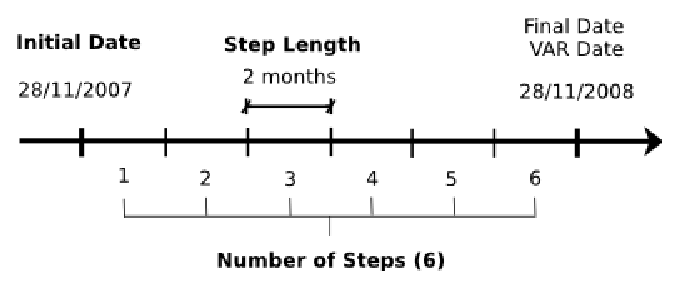
\includegraphics[height=3.0cm, angle=0]{./images/cctime1.eps}
\caption{Time nodes}
\label{cctime1}
\end{center}
\end{figure}
\FloatBarrier

%---------------------------------------------------------------------------
\subsection{Ratings and Survival Functions}
A rating tells a lender or investor the probability of the subject being 
able to pay back a loan. A poor rating indicates a high risk of defaulting.
Every rating has a survival function associated. This function indicates the 
probability that a borrower with initial rating $X$ be non-defaulted at time $t$.
The creation of a rating system and the construction of the survival functions are 
outside the scope of this paper\footnote{Appendix \ref{ap:tmatrix} shows 
how to determine the survival functions using the transition matrix.}.

\begin{figure}[!hbt]
\begin{center}
\includegraphics[height=10cm, angle=-90]{./images/survival.ps}
\caption{Survival functions}
\label{survival}
\end{center}
\end{figure}
\FloatBarrier

%---------------------------------------------------------------------------
\subsection{Sectors and Correlations}
\label{sectors}
The risk of a credit portfolio depends crucially on default correlations between 
economic sectors. These sectors are groupings of companies that react similarly to 
given economic conditions. Example of sectors: energy, financial, technology, 
media and entertainment, utilities, health care, etc. Default correlations between 
sectors measures the default dependence between the defined sectors. This can 
be expressed in tabular form:

\begin{center}
\begin{tabular}[]{cc}
\begin{tabular}[]{c|ccc}
             & $Sector_1$   & $\dots$  & $Sector_{m}$ \cr
\hline
$Sector_1$   & $\rho_{1,1}$ & $\dots$  & $\rho_{1,m}$ \cr
$\vdots$     & $\vdots$     & $\ddots$ & $\vdots$     \cr
$Sector_{m}$ & $\rho_{1,m}$ & $\dots$  & $\rho_{m,m}$ \cr
\end{tabular}
&
\qquad $\rho_{i,j} = Corr(Sector_i, Sector_j)$
\end{tabular}
\end{center}

How to fix the $\rho_{i,j}$ values is outside the scope of this paper.

%---------------------------------------------------------------------------
\subsection{Portfolio}
Portfolio is composed by borrowers. Each borrower has an initial rating and 
belongs to a sector. Each borrower have one or more assets. Each asset
is defined by its addition date in the portfolio, expected cashflow and 
forecasted recovery at certain dates. Figure \ref{portfolio} shows the 
structure of a portfolio.

\begin{figure}[!hbt]
\begin{center}
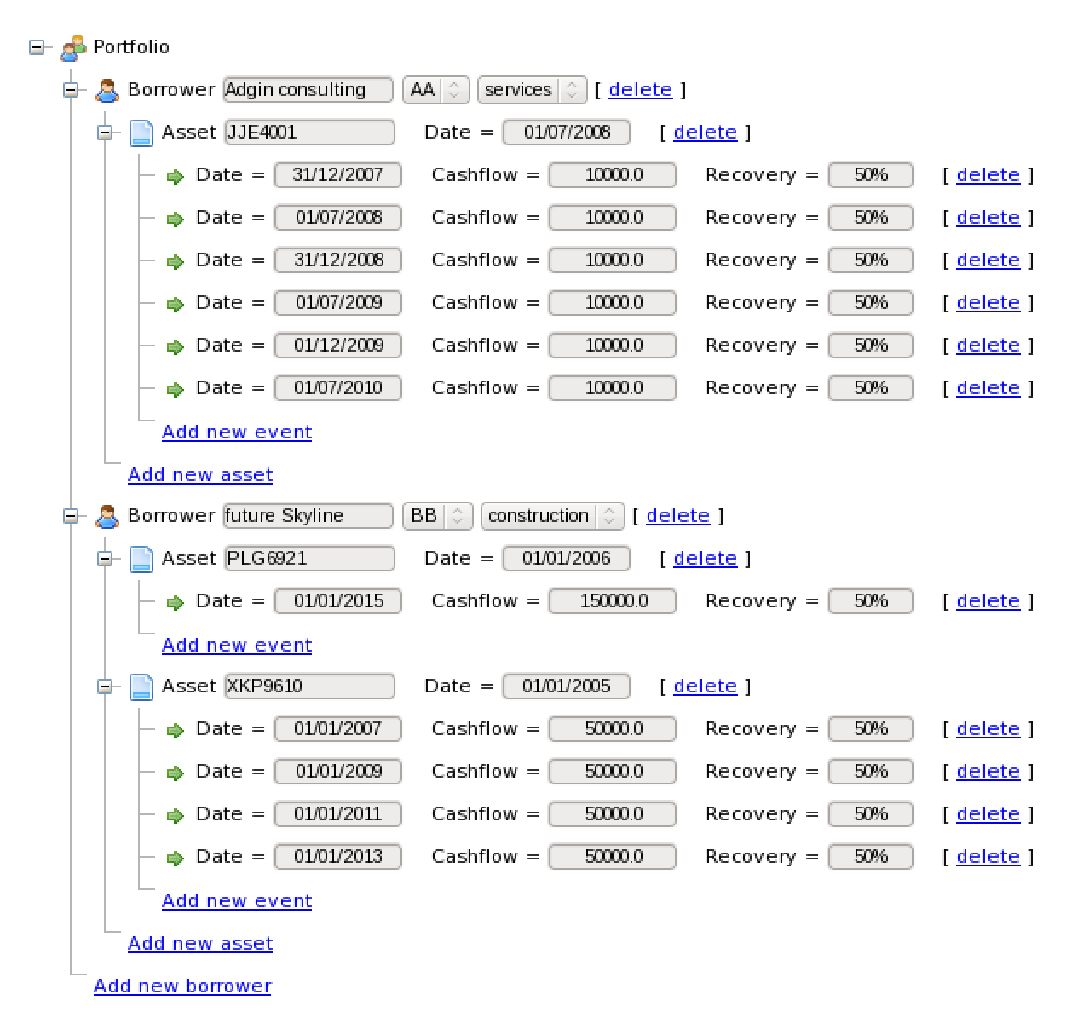
\includegraphics[height=11cm, angle=0]{./images/portfolio.eps}
\caption{Portfolio example}
\label{portfolio}
\end{center}
\end{figure}
\FloatBarrier

\emph{Cashflow} indicates the cash given to the borrower (negative amounts) and the
cash received from the borrower (positive amounts) at each date (see figure \ref{cashflow}).

\begin{figure}[!hbt]
\begin{center}
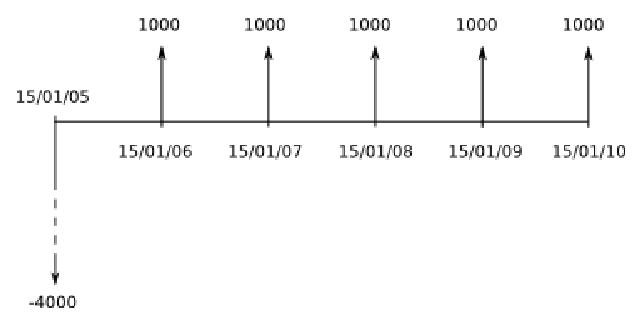
\includegraphics[width=7cm, angle=0]{./images/cashflow.eps}
\caption{Asset cashflow example}
\label{cashflow}
\end{center}
\end{figure}
\FloatBarrier

\emph{Recovery} indicates the cash recovered (after taking legal action against the 
borrower) if the borrower defaults at a certain date (see figure \ref{recovery}).

\begin{figure}[!hbt]
\begin{center}
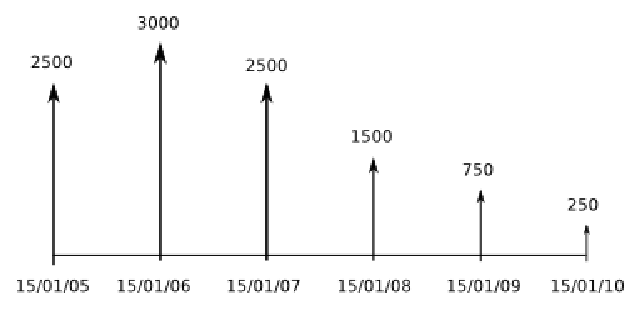
\includegraphics[width=7cm, angle=0]{./images/recovery.eps}
\caption{Asset recovery example}
\label{recovery}
\end{center}
\end{figure}
\FloatBarrier

If a borrower defaults, the loss due to this default is the sum of all remaining
cashflows at default time minus the recovery at default time.


%===========================================================================
\clearpage
\section{Resolution}

This section explains how CCruncher computes the credit risk of a portfolio.

\begin{figure}[!hb]
\begin{center}
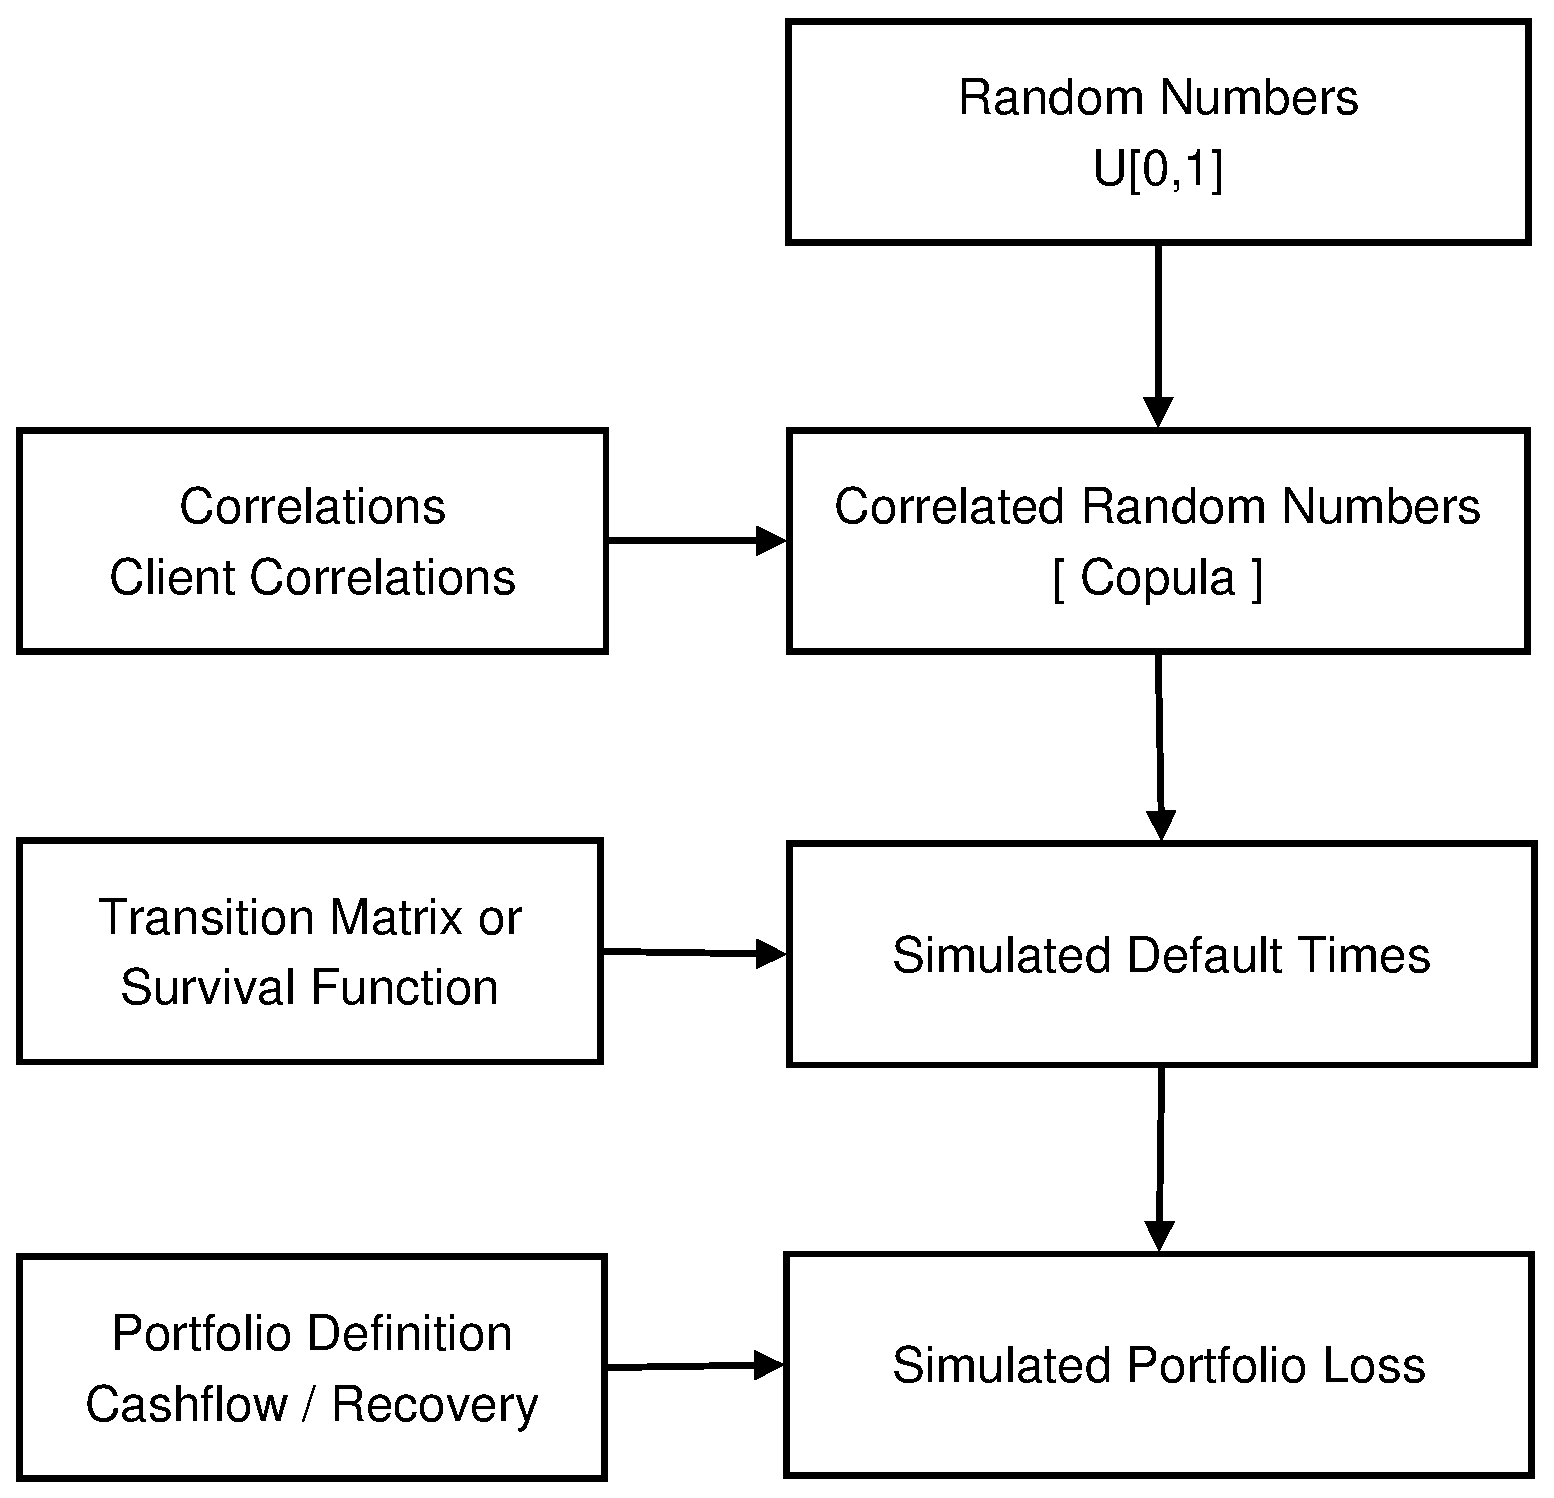
\includegraphics[width=10cm,angle=0]{./images/esquema1.eps}
\caption{Monte Carlo simulation schema}
\label{fig:mcschema1}
\end{center}
\end{figure}

%---------------------------------------------------------------------------
\subsection{Borrowers correlation matrix}
\label{tcorrel}
We need to translate from default correlations between sectors to default 
correlations between borrowers. Let us suppose that we have $n$ borrowers and $m$ 
sectors. Each borrower belongs to a sector. Correlations between sectors are 
known (see \ref{sectors}):

\begin{center}
\begin{tabular}[]{cc}
\begin{tabular}[]{c|ccc}
             & $Sector_1$   & $\dots$  & $Sector_{m}$ \cr
\hline
$Sector_1$   & $\rho_{1,1}$ & $\dots$  & $\rho_{1,m}$ \cr
$\vdots$     & $\vdots$     & $\ddots$ & $\vdots$     \cr
$Sector_{m}$ & $\rho_{1,m}$ & $\dots$  & $\rho_{m,m}$ \cr
\end{tabular}
&
\qquad $\rho_{i,j} = Corr(Sector_i, Sector_j)$
\end{tabular}
\end{center}

We sort the borrowers so that we find those of sector $1$ at the beginning and
those of sector $m$ at the end. Then we create the borrowers correlation matrix 
taking as correlation between two borrowers the correlation between their sectors
(see figure \ref{borrowercorrel}).

\begin{figure}[!hb]
\begin{displaymath}
\begin{array}{c}
\left(
\begin{array}{ccccccccccc}
1           & \dots    & \rho_{1,1}  &          & \rho_{1,k}  & \dots   & \rho_{1,k}  &         & \rho_{1,m}  & \dots      & \rho_{1,m}  \cr
\vdots      & \ddots   & \vdots      &          & \vdots      &         & \vdots      &         & \vdots      &            & \vdots      \cr
\rho_{1,1}  & \dots    & 1           &          & \rho_{1,k}  & \dots   & \rho_{1,k}  &         & \rho_{1,m}  & \dots      & \rho_{1,m}  \cr

            &          &             & \ddots   &             &         &             &         &             &            &             \cr

\rho_{1,k}  & \dots    & \rho_{1,k}  &          & 1           & \dots   & \rho_{k,k}  &         & \rho_{k,m}  & \dots      & \rho_{k,m}  \cr
\vdots      & \ddots   & \vdots      &          & \vdots      & \ddots  & \vdots      &         & \vdots      &            & \vdots      \cr
\rho_{1,k}  & \dots    & \rho_{1, }  &          & \rho_{k,k}  & \dots   & 1           &         & \rho_{k,m}  & \dots      & \rho_{k,m}  \cr

            &          &             &          &             &         &             & \ddots  &             &            &             \cr

\rho_{1,m}  & \dots    & \rho_{1,m}  &          & \rho_{k,m}  & \dots   & \rho_{k,m}  &         & 1           & \dots      & \rho_{m,m}  \cr
\vdots      & \ddots   & \vdots      &          & \vdots      & \ddots  & \vdots      &         & \vdots      & \ddots     & \vdots      \cr
\rho_{1,m}  & \dots    & \rho_{1,m}  &          & \rho_{k,m}  & \dots   & \rho_{k,m}  &         & \rho_{m,m}  & \dots      & 1           \end{array}
\right)
\end{array}
\end{displaymath}
\caption{Borrowers correlation matrix}
\label{borrowercorrel}
\end{figure}

Observe that this is a correlation matrix (symmetric, definite positive, 
$|\rho_{i,j}| < 1$, $|\rho_{i,i}| = 1$) composed by blocks. We will use this 
characteristic to adapt the Cholesky algorithm with the aim to improve memory 
size and speed.

%---------------------------------------------------------------------------
\subsection{Mapping asset losses at fixed time nodes}
Fixed time nodes can be different from cashflow dates. Because we want CCruncher 
to be fast in performing Monte Carlo simulation we precompute the losses of each 
asset at fixed time nodes. The following paragraphs tell how to compute losses at 
fixed time nodes.

%...........................................................................
\subsubsection{Asset recovery at fixed time nodes}
We consider the recovery at time node $k$ as the closest asset recovery by 
right. If time node $k$ is previous to the first asset event then the recovery 
value at time node $k$ is $0$. If time node $k$ is later to the last asset event 
then the recovery value at time node $k$ is $0$. Figure \ref{recoverymapping} 
shows the recoveries displayed in figure \ref{recovery} mapped to, in this case,
half-yearly time nodes.

\begin{figure}[!hbtp]
\begin{center}
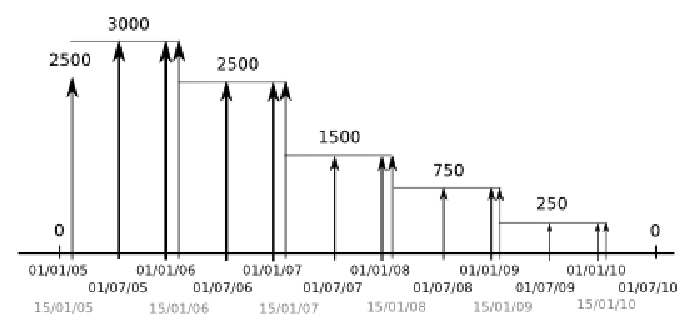
\includegraphics[width=12cm, angle=0]{./images/recoverymapping.eps}
\caption{Asset recoveries mapped to fixed time nodes}
\label{recoverymapping}
\end{center}
\end{figure}
\FloatBarrier

%...........................................................................
\subsubsection{Asset losses at fixed time nodes}
If borrower defaults before the date of asset risk assumption then loss is $0$.
If borrower defaults after asset finalization date then loss is $0$. 
If borrower defaults at time node $k$ then loss is the averaged sum of all 
pending cashflows minus the recovery at time node $k$.
Figure \ref{lossesmapping} shows asset losses mapped to, in this case, half-yearly 
time nodes of the asset displayed in figures \ref{cashflow}, \ref{recovery} and 
\ref{recoverymapping}.

\begin{figure}[!hbtp]
\begin{center}
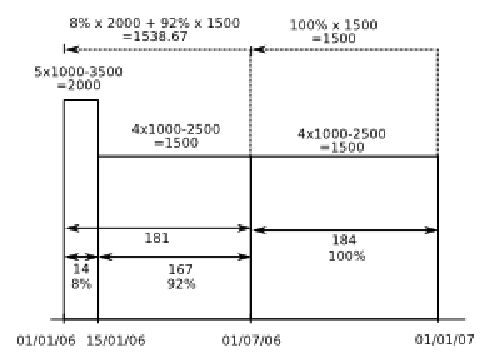
\includegraphics[width=7.34cm, angle=0]{./images/lossesmapping.eps}
\caption{Asset losses mapped to time nodes 01/07/06 and 01/01/07}
\label{lossesmapping}
\end{center}
\end{figure}
\FloatBarrier

%---------------------------------------------------------------------------
\subsection{Monte Carlo simulation}
\label{mcsim}
Monte Carlo methods \cite{mc:mervyn} are a class of computational algorithms for 
simulating the behavior of various physical and mathematical systems. 
Each simulation consists of computing a random default time for each borrower and
then calculate the loss of the portfolio. We need that default times fulfill two 
conditions: the borrower's survival functions and the borrower's correlation matrix. 
This is achieved by simulating a copula. A copula \cite{copu:pitfalls} 
\cite{copu:wang} is a multivariate random variable where each component is a 
uniform $U[0,1]$. Lets go step by step:

%...........................................................................
\subsubsection{Random numbers generation}
Each simulation requires a set of random numbers between $[0, 1]$ and correlated 
by the borrowers' correlation matrix, $\Sigma_1$ (see \ref{tcorrel}, figure 
\ref{borrowercorrel}). We generate these numbers using the gaussian copula simulation 
algorithm:

\paragraph{Step 1.} We create the covariance\footnote{Correlation and covariance 
matrix are the same because diagonal elements are $1$.} matrix $\Sigma_2$ mapping 
$\Sigma_1$ component by component:
\begin{displaymath}
\Sigma_2 = \left( 
\begin{array}{cccc}
2 sin(\frac{\pi}{6})           & 2 sin(\rho_{12} \frac{\pi}{6}) & \ldots & 2 sin(\rho_{1n} \frac{\pi}{6})\cr
2 sin(\rho_{12} \frac{\pi}{6}) & 2 sin(\frac{\pi}{6})           & \ldots & 2 sin(\rho_{2n} \frac{\pi}{6})\cr
\vdots                         & \vdots                         & \ddots  & \vdots   \cr
2 sin(\rho_{1n} \frac{\pi}{6}) & 2 sin(\rho_{2n} \frac{\pi}{6}) & \ldots & 2 sin(\frac{\pi}{6})
\end{array}
\right)
\end{displaymath}
Observe that $\Sigma_2$ have diagonal elements with $1$ because $2 sin(\frac{\pi}{6}) = 1$.

\paragraph{Step 2.} We apply Cholesky to $\Sigma_2$, then $\Sigma_2 = B \cdot B^{\top}$, 
where:
\begin{displaymath}
B = 
\left(
\begin{array}{cccc}
b_{11}   & 0        & \ldots & 0       \cr
b_{21}   & b_{22}   & \ldots & 0       \cr
\vdots  & \vdots  & \ddots & \vdots \cr
b_{n1}   & b_{n2}   & \ldots & b_{nn}
\end{array}
\right)
\end{displaymath}

\paragraph{Step 3.} We simulate\footnote{The algorithm used to simulate a $N(0,1)$
is explained in appendix \ref{ap:normsim}} a $N(0,1)$ $n$ times:
\begin{displaymath}
\vec{Y} =
\left(
\begin{array}{c}
y_1 \cr
\vdots \cr
y_n
\end{array}
\right) 
\qquad y_k \sim N(0,1) \textrm{ independents}
\end{displaymath}

\paragraph{Step 4.} We simulate a normal multivariate $\vec{Z} \sim N(\vec{0}, \Sigma_2)$ 
doing:
\begin{displaymath}
B \cdot \vec{Y} 
=
\left(
\begin{array}{cccc}
b_{11}   & 0        & \ldots & 0       \cr
b_{21}   & b_{22}   & \ldots & 0       \cr
\vdots  & \vdots  & \ddots & \vdots \cr
b_{n1}   & b_{n2}   & \ldots & b_{nn}
\end{array}
\right)
\left(
\begin{array}{c}
y_1 \cr
\vdots \cr
y_n
\end{array}
\right) 
=
\left(
\begin{array}{c}
z_1 \cr
\vdots \cr
z_n
\end{array}
\right) 
= 
\vec{Z}
\end{displaymath}

\paragraph{Step 5.} Finally we obtain the copula $\vec{U}$ doing:
\begin{displaymath}
\left(
\begin{array}{c}
\Phi(z_1) \cr
\vdots \cr
\Phi(z_n)
\end{array}
\right) 
=
\left(
\begin{array}{c}
u_1 \cr
\vdots \cr
u_n
\end{array}
\right) 
=
\vec{U} 
\end{displaymath}
where $\Phi(x)$ is the $N(0,1)$ cumulative distribution function.
\begin{displaymath}
\Phi(x) = \int_{-\infty}^{x} \frac{1}{\sqrt{2 \pi}} e^{-\frac{t^2}{2}} dt
\end{displaymath}

Steps 1 and 2 are done only one time before the simulations. The rest of steps
are performed in each Monte Carlo simulation.
\newline

In appendix \ref{ap:cholblock} is described a Cholesky decomposition adapted to 
block matrix. It allows to work with matrix bigger than $50000 \times 50000$.

%...........................................................................
\subsubsection{Default times generation}
Given the borrower $k$ and the random number $u_k \in [0,1]$ (generated using a 
copula in the previous step) we simulate the default time considering the 
inverse of the borrower survival function at $u_k$. Figure \ref{simttd} shows 
this in a graphic manner.

\begin{figure}[!hbt]
\begin{center}
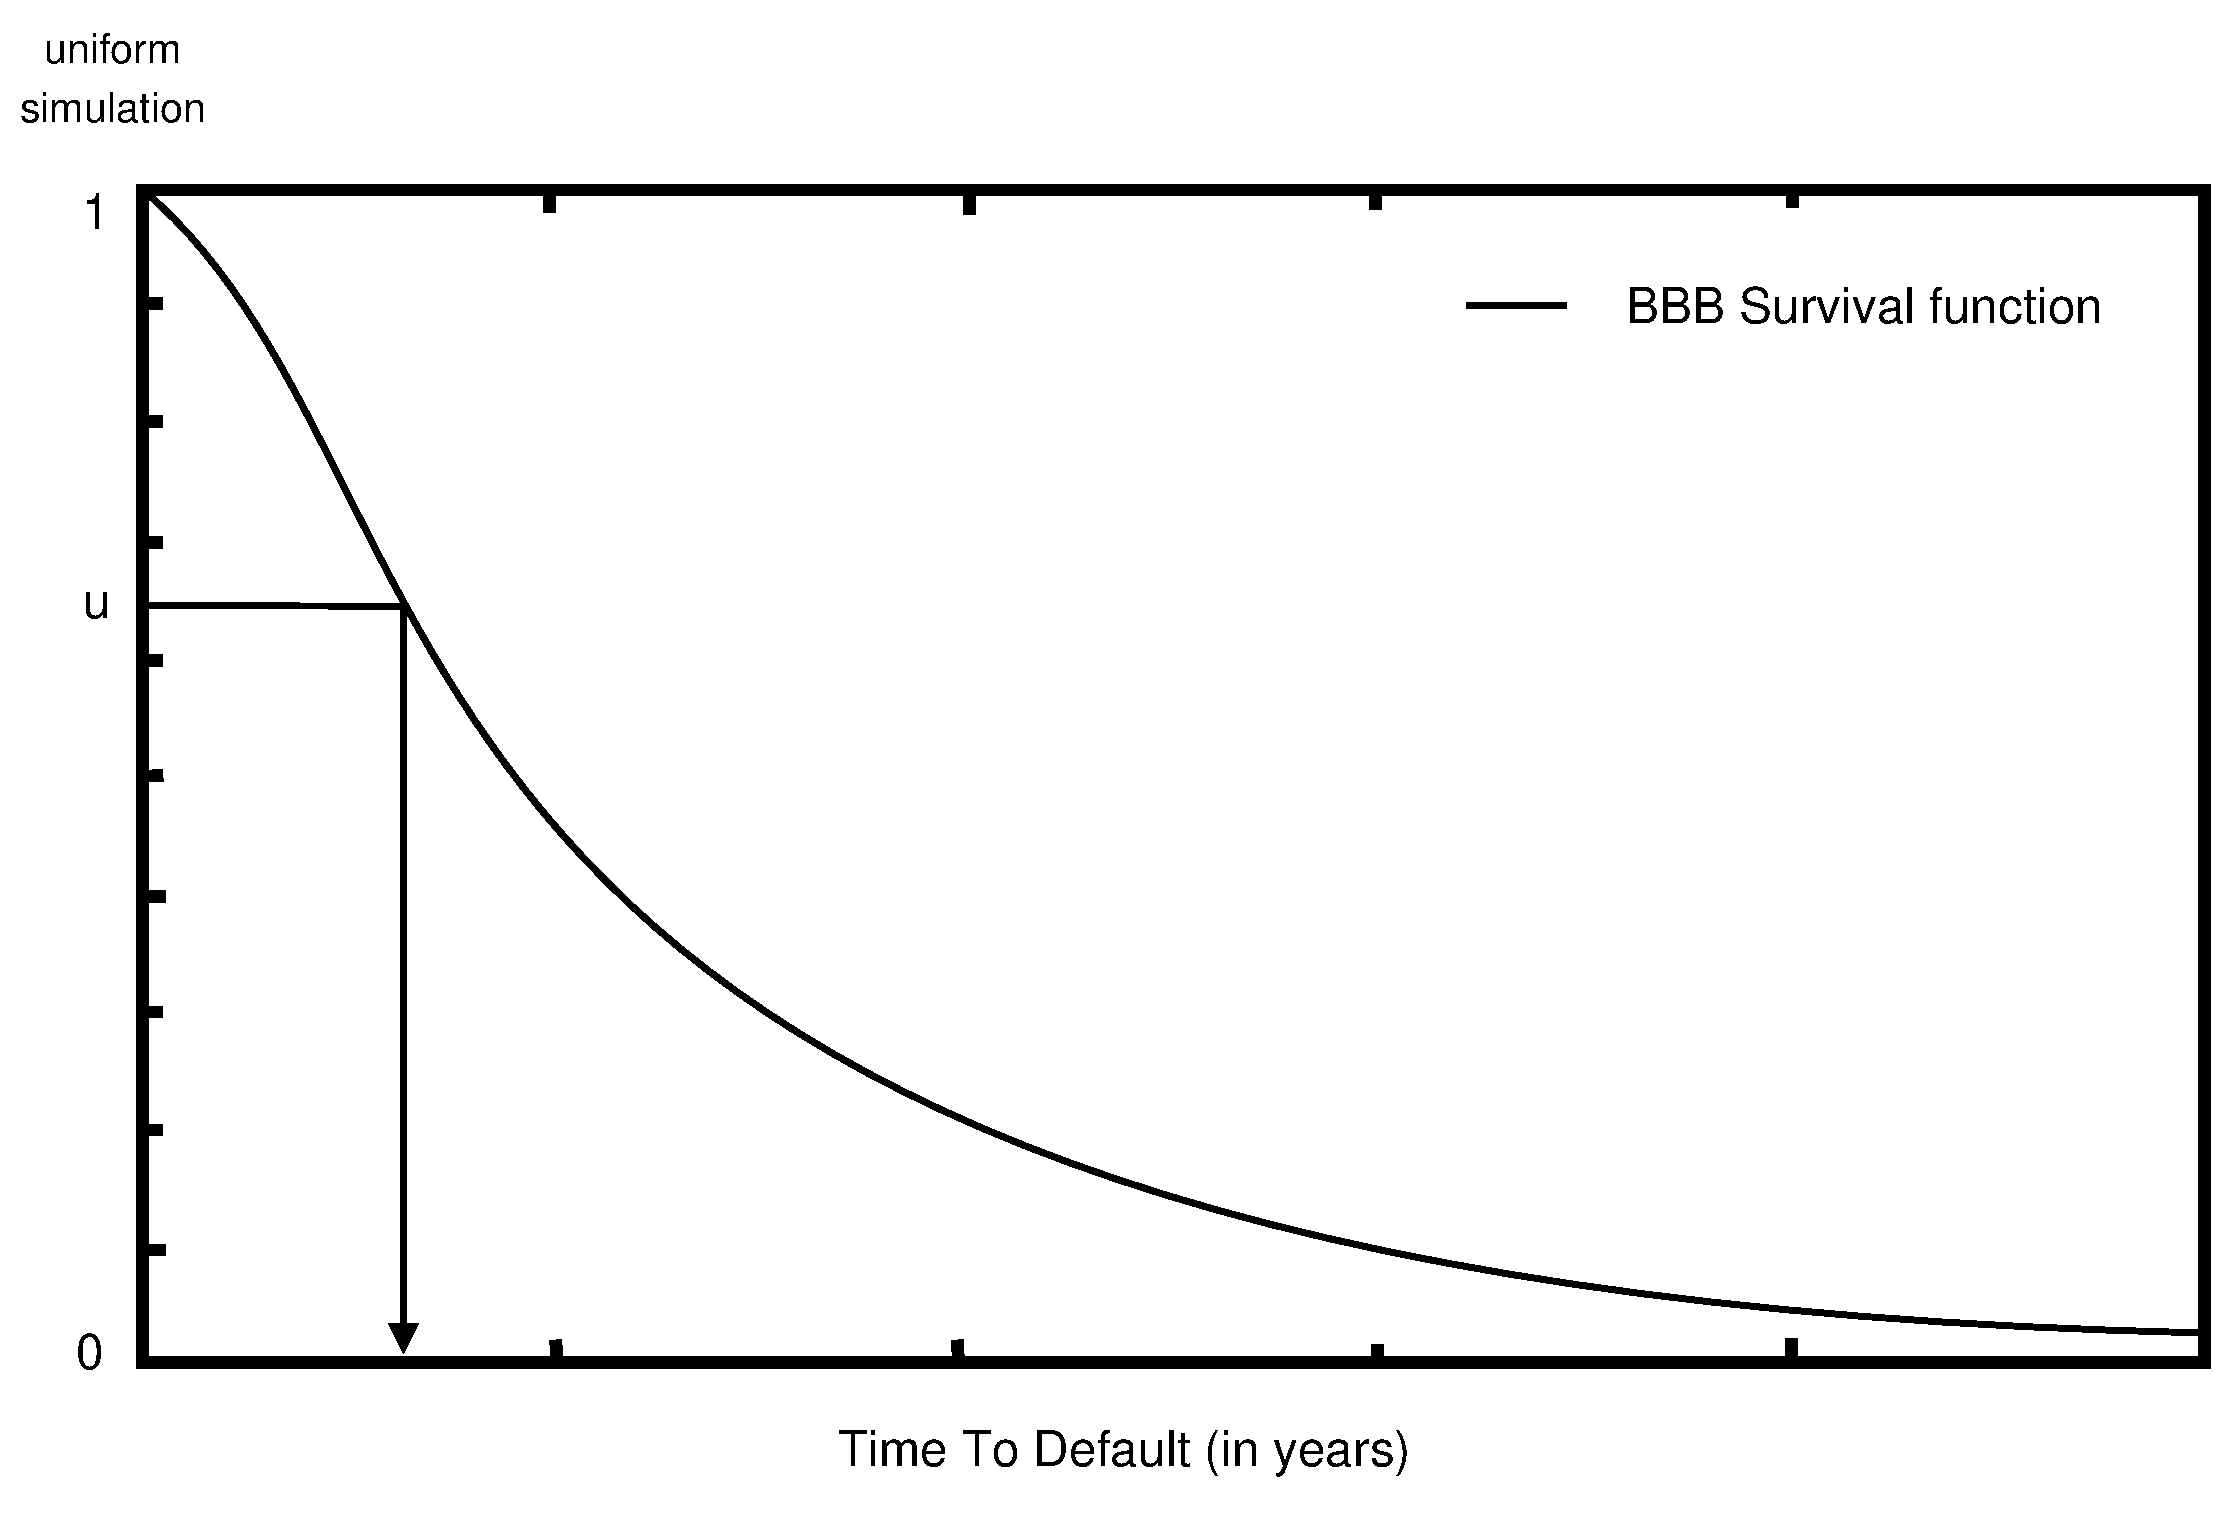
\includegraphics[width=10cm,angle=0]{./images/simttd.eps}
\caption{Default time generation with initial rating $BBB$}
\label{simttd}
\end{center}
\end{figure}
\FloatBarrier

%...........................................................................
\subsubsection{Portfolio loss evaluation}
At this point, given any borrower, we have a simulated default time. We map
this default time to the closest time node to the right. In this node we have 
the precomputed losses of that borrower's assets. To obtain the simulated 
value of the portfolio loss we sum all asset losses and we keep this value 
in a list. Afterwards we will use this list to compute risk.

%---------------------------------------------------------------------------
\subsection{Risk computation}
After $N$ simulations (eg. $20000$, $50000$ or more) we have a list
of numbers, ${x_1, ..., x_N}$, where each number represents a simulated portfolio 
loss. The more values, the more accuracy in the results. All risk statistics (eg. 
Expected Loss) have an error margin that will be estimated. CCruncher uses 
\emph{R package}\footnote{http://www.r-project.org} to perform the statistical
computations described below.
\newline

First of all we can approximate the probability distribution of the portfolio 
loss creating an histogram with the simulated values.

\begin{figure}[!hbt]
\begin{center}
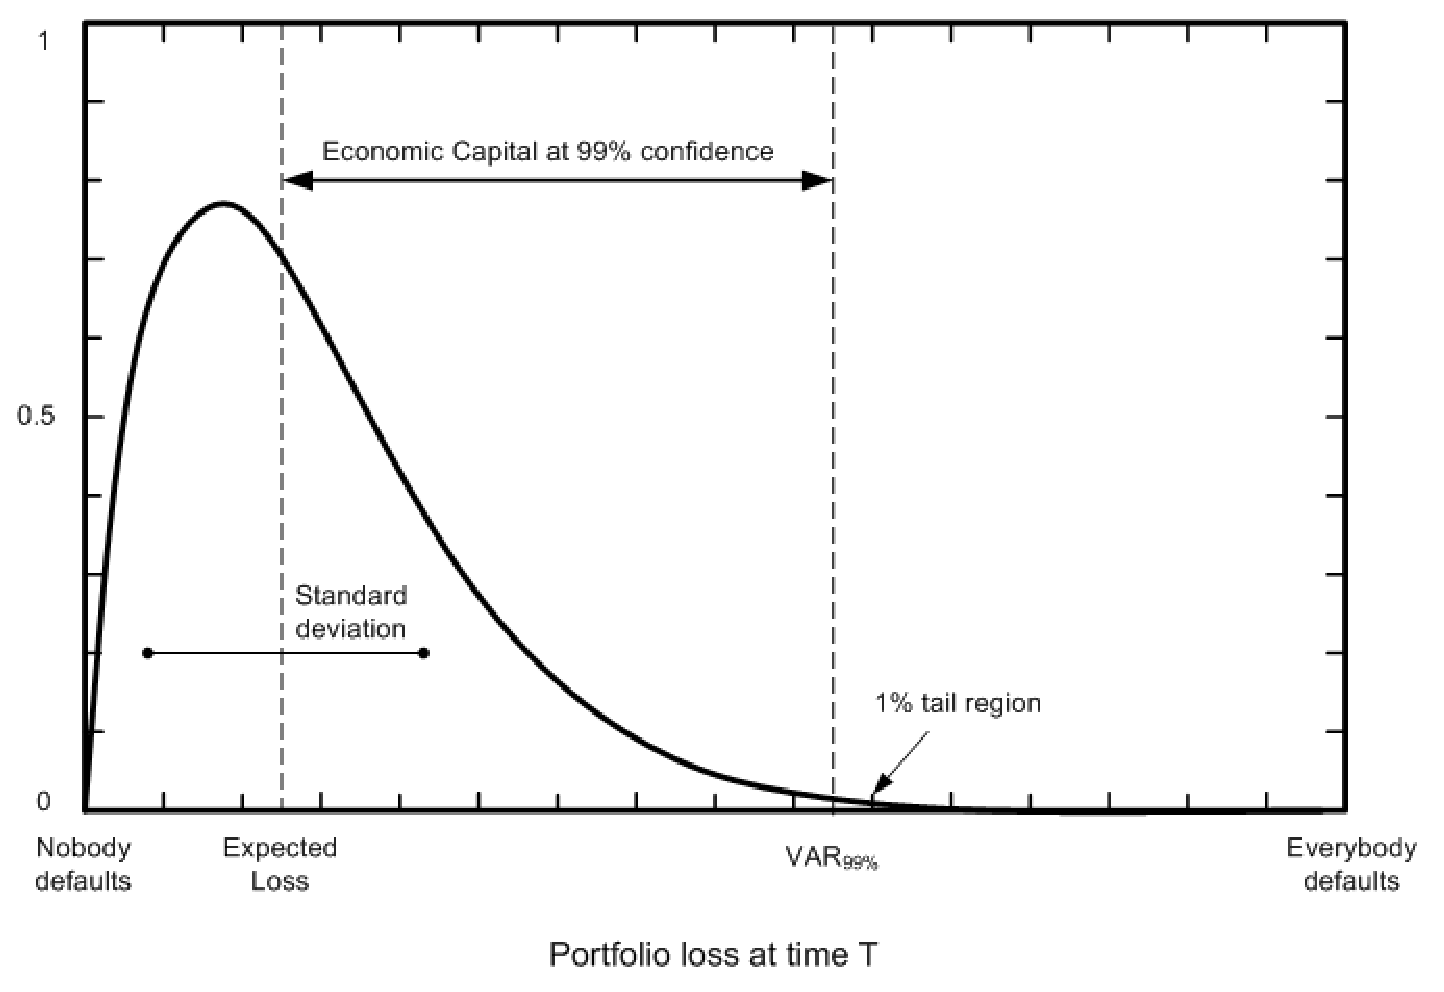
\includegraphics[height=7cm, angle=0]{./images/creditvar.eps}
\caption{Portfolio loss at time $T$}
\label{creditvar}
\end{center}
\end{figure}
\FloatBarrier

%...........................................................................
\subsubsection{Expected Loss}
Expected Loss is the probability distribution mean of the portfolio loss.
Central Limit Theorem \cite{stats:schaum} grants that:

\begin{displaymath}
\mu = \widehat{\mu} \pm \phi^{-1}\left(\frac{1-\alpha}{2}\right) \cdot \frac{\widehat{\sigma}}{\sqrt{N}}
\end{displaymath}
where $\alpha$ is the error confidence level, $\phi^{-1}$ the N(0,1) inverse 
cumulative distribution function and $\widehat{\mu}$ and $\widehat{\sigma}$ are 
the mean and stddev estimators:

\begin{displaymath}
\widehat{\mu} = \frac{1}{N} \sum_{i=1}^{N} x_i
\end{displaymath}

\begin{displaymath}
\widehat{\sigma} =
\sqrt{\frac{1}{N-1} \sum_{i=1}^{N} \left( x_i - \widehat{\mu} \right)^2} =
\sqrt{\frac{1}{N-1} \left( \sum_{i=1}^{N} x_i^2 - \frac{\left(\sum_{i=1}^{N} x_i \right)^2}{N} \right)}
\end{displaymath}

%...........................................................................
\subsubsection{Portfolio Loss Standard Deviation}
Another usual risk statistic is the standard deviation of the portfolio loss.
Central Limit Theorem \cite{stats:schaum} grants that:

\begin{displaymath}
\sigma = \widehat{\sigma} \pm \phi^{-1}\left(\frac{1-\alpha}{2}\right) \cdot \frac{\widehat{\sigma}}{\sqrt{2N}}
\end{displaymath}

where $\alpha$ is the error confidence level, $\phi^{-1}$ the N(0,1) inverse 
cumulative distribution function and $\widehat{\sigma}$ is the stddev estimator:

\begin{displaymath}
\widehat{\sigma} =
\sqrt{\frac{1}{N-1} \sum_{i=1}^{N} \left( x_i - \widehat{\mu} \right)^2} =
\sqrt{\frac{1}{N-1} \left( \sum_{i=1}^{N} x_i^2 - \frac{\left(\sum_{i=1}^{N} x_i \right)^2}{N} \right)}
\end{displaymath}

%...........................................................................
\subsubsection{Value At Risk}
Value at Risk \cite{var:jorion} is the most used risk value. We call it 
$VAR_{\beta}$ where $\beta$ is the VAR confidence level (eg. VAR at $95\%$).
VAR is another form to say quantile. Then
$VAR_{\beta} = q_{\beta} = \textrm{inf}\{x | F(x) \geq \beta \}$. 

\begin{displaymath}
VAR_{\beta} = \widehat{q_{\beta}} \pm \phi^{-1}\left(\frac{1-\alpha}{2}\right) \cdot \textrm{stderr}(q_{\beta})
\end{displaymath}

where $\alpha$ is the error confidence level, $\beta$ is the VAR confidence 
level, $\phi^{-1}$ the N(0,1) inverse cumulative distribution function, 
$\widehat{q_{\beta}}$ is the quantile estimator, and $\textrm{stderr}(q_{\beta})$
is the estimation of the standard error.

\begin{displaymath}
\widehat{q_{\beta}} = x_{k:N}
\end{displaymath}
where,
\begin{itemize}
\item $k$ fulfills $\frac{k}{N} \leq \beta < \frac{k+1}{N}$
\item $x_{k:N}$ is the $k$-th element of ascendent sorted values
\end{itemize}

We determine $\textrm{stderr}(q_{\beta})$ using Maritz-Jarret method described
in \cite{quant:algor}.

\begin{eqnarray}
M   & = & [N \beta + 0.5] \nonumber \\
a   & = & M - 1 \nonumber \\
b   & = & N - M \nonumber \\
W_i & = & B(a,b,\frac{i+1}{N}) - B(a,b,\frac{i}{N}) \nonumber \\
C_k & = & \sum_{i=1}^{N} W_i \cdot x_i \nonumber
\end{eqnarray}

where $[x]$ is the integer part of $x$ and $B(a,b,x)$ is the incomplete beta 
function:

\begin{displaymath}
B(a,b,x)=\frac{\Gamma(a+b)}{\Gamma(a)\Gamma(b)}\int_0^x t^{a-1} (1-t)^{b-1} dt
\end{displaymath}

Then,
\begin{displaymath}
\textrm{stderr}(q_{\beta}) = \sqrt{C_2 - C_1^2}
\end{displaymath}

%...........................................................................
\subsubsection{Expected Shortfall}
VAR is not a distance because it does not fulfill the sub-additive property 
\cite{var:varbad}, $VAR(A+B) \nleq VAR(A)+VAR(B)$. Expected Shortfall is a 
consistent risk measure \cite{var:eshortfall} similar to VAR. It can be described
as the average of the $\beta\%$ worst losses.

\begin{displaymath}
ES_{\beta} = \widehat{ES_{\beta}} \pm \phi^{-1}\left(\frac{1-\alpha}{2}\right) \cdot \textrm{stderr}(ES_{\beta})
\end{displaymath}

where $\alpha$ is the error confidence level, $\beta$ is the ES confidence 
level, $\phi^{-1}$ the N(0,1) inverse cumulative distribution function, 
$\widehat{ES_{\beta}}$ is the ES estimator and $\textrm{stderr}(ES_{\beta})$
is the estimation of the standard error.
\newline

We select the simulation portfolio loss values ($x_1, ..., x_N$) that are bigger 
than $VAR_{\beta}$.

\begin{displaymath}
y_1, y_2, y_3, \cdots, y_K \qquad \textrm{where} \quad y_i > VAR_{\beta}
\end{displaymath}

Then,

\begin{displaymath}
\widehat{ES_{\beta}} = \frac{1}{K} \sum_{i=1}^{K} y_i
\end{displaymath}

\begin{displaymath}
\textrm{stderr}(ES_{\beta}) =
\frac{\sqrt{\frac{1}{K-1} \sum_{i=1}^{K} \left( y_i - \widehat{ES_{\beta}} \right)^2}}{\sqrt{K}} =
\frac{\sqrt{\frac{1}{K-1} \left( \sum_{i=1}^{K} y_i^2 - \frac{\left(\sum_{i=1}^{K} y_i \right)^2}{K} \right)}}{\sqrt{K}}
\end{displaymath}

%...........................................................................
\subsubsection{Economic Capital}
We can compute the Economic Capital at confidence level $\beta$ as:

\begin{displaymath}
\textrm{Economic Capital} = VAR_{\beta} - \textrm{Expected Loss}
\end{displaymath}

%...........................................................................

\begin{figure}[p]
\begin{center}
\includegraphics[width=12cm,angle=0]{./images/report.eps}
\caption{CCruncher results}
\label{report}
\end{center}
\end{figure}


%===========================================================================
\clearpage
\section{Other considerations}
CCruncher takes into consideration other concepts that have not been exposed 
up to this moment with the purpose of simplifying the content.

%---------------------------------------------------------------------------
\subsection{Risk aggregation}
CCruncher simulates the whole portfolio loss at time $T$. It also allows (in 
the same execution) the simulation of subportfolios by defining one or more 
aggregators. Consequently you can determine which are the borrowers (or products 
or branches or regions or assets, etc.) that increase the risk of your portfolio. 
Every subportfolio has its own list of simulated values that can be processed to 
obtain the risk indicators for this subportfolio.

%---------------------------------------------------------------------------
\subsection{Yield curve}
CCruncher can consider that money value decreases along the time following a fixed 
curve (eg. yield curve). CCruncher allows the input of the yield curve and and takes
it into account in all its computations. The coeficient that determines the money 
value decreases along the time is given by the compound interest formula:

\begin{displaymath}
\Upsilon(r, t_0,t_1) = (1+r)^{(t_1-t_0)}
\end{displaymath}

%---------------------------------------------------------------------------
\subsection{Antithetic technique}
The random number generation using a copula is time expensive. Gaussian copula
is symmetric, that means that $(u_1, u_2, \cdots, u_N)$ is equiprobable to
$(1-u_1, 1-u_2, \cdots, 1-u_N)$. In CCruncher's antithetic mode, each copula 
generation is used $2$ times, $(u_1, u_2, \cdots, u_N)$ and 
$(1-u_1, 1-u_2, \cdots, 1-u_N)$, reducing to the half the number of generated
copulas.

%---------------------------------------------------------------------------
\subsection{Parallel computing}
Monte Carlo problems are embarrassingly parallel problems.
In the jargon of parallel computing, an embarrassingly parallel workload 
(or embarrassingly parallel problem) is one for which no particular effort 
is needed to segment the problem into a very large number of parallel tasks, 
and there is no essential dependency (or communication) between those parallel 
tasks.
\newline

In CCruncher the master sends the RNG seed to each slave 
($seed_i = seed + i \cdot 30001$) and waits for results (the simulated values of
the portfolio loss) from slaves that store them in a file. When one of the two stop 
criteria is achieved (maximum execution time exceded or maximum number of 
simulations reached) the master sends a stop signal to the slaves and leaves.

%===========================================================================
\appendix
\section{Appendices}

%---------------------------------------------------------------------------
\subsection{How to simulate a N(0,1)}
\label{ap:normsim}

In order to simulate $Z \sim N(\mu, \sigma^2)$ values we use:

\begin{displaymath}
z = \mu + \sigma\cdot \sqrt{-2 ln(u_1)} \cdot cos(2 \pi \cdot u_2)
\qquad u_1, u_2 \sim U[0,1]
\end{displaymath}

Where $u_i$ are generated by a Mersenne Twister random number generator.

%---------------------------------------------------------------------------
\subsection{Cholesky decomposition for block matrix}
\label{ap:cholblock}

Cholesky algorithm decomposes a symmetric positive definite matrix into a lower
triangular matrix and the transpose of the lower triangular matrix. Algorithm 
description can be found in \emph{Numerical Recipes in C}\footnote{http://www.nr.com}.

\begin{displaymath}
A = U^{\top} \cdot U
\end{displaymath}

If we have a portfolio of $50000$ borrowers, the correlation matrix size will
be a $50000 \times 50000$. This requires up to 19 Gb. of RAM memory. The 
multiplication of this matrix by a vector implies $2500000000$ multiplications.
This is far too much. So we adapt the Cholesky algorithm in order to consider that 
the borrowers' correlation matrix is a block matrix with $1$'s in diagonal. 
For instance:

\begin{displaymath}
A = \left(
\begin{array}{cccc|ccc}
1   & 0.5 & 0.5 & 0.5 & 0.1 & 0.1 & 0.1 \cr
0.5 & 1   & 0.5 & 0.5 & 0.1 & 0.1 & 0.1 \cr
0.5 & 0.5 & 1   & 0.5 & 0.1 & 0.1 & 0.1 \cr
0.5 & 0.5 & 0.5 & 1   & 0.1 & 0.1 & 0.1 \cr
\hline
0.1 & 0.1 & 0.1 & 0.1 & 1   & 0.3 & 0.3 \cr
0.1 & 0.1 & 0.1 & 0.1 & 0.3 & 1   & 0.3 \cr
0.1 & 0.1 & 0.1 & 0.1 & 0.3 & 0.3 & 1
\end{array}
\right)
\end{displaymath}

We decompose the previous matrix using the standard Cholesky decomposition:

\begin{displaymath}
U = \left(
\begin{array}{cccc|ccc}
 1.00000 & 0.50000 & 0.50000 & 0.50000 & 0.10000 & 0.10000 & 0.10000 \cr
 0       & 0.86603 & 0.28868 & 0.28868 & 0.05774 & 0.05774 & 0.05774 \cr
 0       & 0       & 0.81650 & 0.20412 & 0.04082 & 0.04082 & 0.04082 \cr
 0       & 0       & 0       & 0.79057 & 0.03162 & 0.03162 & 0.03162 \cr
\hline
 0       & 0       & 0       & 0       & 0.99197 & 0.28630 & 0.28630 \cr
 0       & 0       & 0       & 0       & 0       & 0.94975 & 0.21272 \cr
 0       & 0       & 0       & 0       & 0       & 0       & 0.92563
\end{array}
\right)
\end{displaymath}

We can see that $U$ have repeated elements that can be kept in RAM memory in 
this way:

\begin{displaymath}
U = \left|
\begin{array}{c|cc}
 1.00000 & 0.50000 & 0.10000 \cr
 0.86603 & 0.28868 & 0.05774 \cr
 0.81650 & 0.20412 & 0.04082 \cr
 0.79057 & 0       & 0.03162 \cr
 0.99197 & 0       & 0.28630 \cr
 0.94975 & 0       & 0.21272 \cr
 0.92563 & 0       & 0
\end{array}
\right|
\end{displaymath}

that is, for each row we keep the diagonal value and the value of each sector. 
With this strategy the required memory size is $N \times (M+1)$ where $N$ is
the number of borrowers and $M$ the number of sectors. With this consideration
the memory required to store a $50000 \times 50000$ borrowers correlation matrix
is only $4.2$ Mb.
\newline

We use the fact that matrix $U$ have repeated elements to reduce the number of 
operations required to multiply $U$ by a vector. Let see an example:

\begin{displaymath}
\begin{array}{l}
(U \cdot x)_2 =  0.86603 \cdot x_2 + 0.28868 \cdot x_3 + 0.28868 \cdot x_4 + \cr
                 0.05774 \cdot x_5 + 0.05774 \cdot x_6 + 0.05774 \cdot x_7 \cr
              = 0.86603 \cdot x_2 + 2\cdot 0.28868 \cdot (x_3 + x_4) + 3 \cdot 0.05774 \cdot (x_5 + x_6 + x_7)
\end{array}
\end{displaymath}

Considering this, we can reduce the number of operations from $N^2$ to 
$N \times (M+1)$ where $N$ is the number of borrowers and $M$ the number of 
sectors. In the $50000$ borrowers example, the operations number reduces from 
$2500000000$ to only $500000$.

%---------------------------------------------------------------------------
\subsection{From transition matrix to survival functions}
\label{ap:tmatrix}
The $T$-years transition matrix gives the probability to jump from rating $r_i$ 
to rating $r_j$ in a term of $T$ years.

\begin{displaymath}
M_T = \left(
\begin{array}{ccc}
m_{1,1} & \dots  & m_{1,n} \cr
\vdots & \ddots & \vdots \cr
m_{n,1} & \dots  & m_{n,n} 
\end{array}
\right)
\qquad
m_{i,j} = P(r_i \to r_j;T)
\end{displaymath}

where $n$ is the number of ratings and $m_{i,j}$ is the probability that a
borrower with rating $r_i$ jumps to $r_j$ in $T$ years.
Figure \ref{tmatrix1} shows a transition matrix example where the probability 
that a borrower with rating $AA$ jumps to rating $B$ in $1$ year is $0.14\%$.
\newline

\begin{figure}[!hb]
\begin{center}
\begin{tabular}[]{l|rrrrrrrr}
        &      AAA &       AA &        A &      BBB &       BB &        B &      CCC &  Default \cr
\hline
AAA     &  $90.81$ &   $8.33$ &   $0.68$ &   $0.06$ &   $0.12$ &   $0.00$ &   $0.00$ &   $0.00$ \cr
 AA     &   $0.70$ &  $90.65$ &   $7.79$ &   $0.64$ &   $0.06$ &   $0.14$ &   $0.02$ &   $0.00$ \cr
  A     &   $0.09$ &   $2.27$ &  $91.05$ &   $5.52$ &   $0.74$ &   $0.26$ &   $0.01$ &   $0.06$ \cr
BBB     &   $0.02$ &   $0.33$ &   $5.95$ &  $86.93$ &   $5.30$ &   $1.17$ &   $0.12$ &   $0.18$ \cr
 BB     &   $0.03$ &   $0.14$ &   $0.67$ &   $7.73$ &  $80.53$ &   $8.84$ &   $1.00$ &   $1.06$ \cr
  B     &   $0.00$ &   $0.11$ &   $0.24$ &   $0.43$ &   $6.48$ &  $83.46$ &   $4.07$ &   $5.21$ \cr
CCC     &   $0.22$ &   $0.00$ &   $0.22$ &   $1.30$ &   $2.38$ &  $11.24$ &  $64.86$ &  $19.78$ \cr
Default &   $0.00$ &   $0.00$ &   $0.00$ &   $0.00$ &   $0.00$ &   $0.00$ &   $0.00$ & $100.00$
\end{tabular}
\caption{$1$-year transition matrix}
\label{tmatrix1}
\end{center}
\end{figure}

Transition matrix can be scaled in time using the following rules:

\begin{equation}
\label{sttm}
\begin{array}{l}
M_{T_1+T_2} = M_{T_1} \cdot M_{T_2} \nonumber \\
M_{k \cdot T} = M_{T}^k \nonumber \\
M_{\frac{T}{k}} = \sqrt[k]{M_{T}} \nonumber
\end{array}
\end{equation}

The root of a matrix can be computed as:

\begin{displaymath}
M = P^{-1} \cdot D \cdot P 
\longrightarrow
M^{\gamma} = P^{-1} \cdot D^{\gamma} \cdot P
\end{displaymath}

where $P$ is a matrix composed by the eigenvectors of $M$ and $D$ is a diagonal 
matrix composed by the eigenvalues of $M$. The inverse of a matrix can be 
computed using the $LU$ decomposition as it is explained in \emph{Numerical 
Recipes in C}\footnote{http://www.nr.com}:

\begin{displaymath}
Id = P^{-1} \cdot P = L \cdot U \cdot P
\end{displaymath}

This allows us to compute default probability at any time and at any initial 
rating (that is, the survival functions), doing:

\begin{displaymath}
Survival(r_i, t) = \left( M_t \right)_{i, n}
\end{displaymath}

where $r_i$ is the initial rating, $t$ is the time, $M_t$ is the transition 
matrix for time $t$ (scaled from $M_T$ using (\ref{sttm})) and $n$ is the 
index of default rating $r_n$.

%===========================================================================
\bibliography{refs}
\bibliographystyle{plain}


\end{document}

